\documentclass[UTF8,a4paper,12pt]{ctexart}
\usepackage[left=2.4cm,right=2.4cm,top=2.5cm,bottom=2.5cm]{geometry}
\usepackage{graphicx}
\usepackage{booktabs}
\usepackage{float}
\usepackage{hyperref}
\usepackage{setspace}
\setstretch{1.25}

\title{大数据原理与技术 作业5实验报告\\股票价格预测：ARIMA 与 LSTM 对比}
\author{姓名：梁力航 \quad 学号：23336128}
\date{2026-03-30}

\begin{document}
\maketitle

\section{实验目的}
本实验围绕单变量股票收盘价序列预测任务，使用同一份历史价格数据分别构建 ARIMA 与 LSTM 模型，并完成测试集评估与未来 7 个交易日预测。实验目标包括：
\begin{enumerate}
    \item 完成从本地 CSV 读取、清洗、切分到训练、预测、评估的一体化流水线；
    \item 在同一测试集上使用 MAE 与 RMSE 对 ARIMA 和 LSTM 的效果进行比较；
    \item 生成图表与表格，支撑模型效果分析；
    \item 产出可提交的代码、结果文件与 PDF 报告。
\end{enumerate}

\section{数据集与实验环境}
\subsection{数据集说明}
实验数据为 Apple 股票历史价格公开 CSV，经清洗后保留：
\begin{itemize}
    \item \texttt{date}：交易日期
    \item \texttt{close}：收盘价
\end{itemize}

本次实验仅使用收盘价单变量序列建模，避免引入题目未要求的复杂特征工程，符合 KISS / YAGNI 原则。

\subsection{实验环境}
\begin{itemize}
    \item 操作系统：macOS
    \item Python 环境：Anaconda \texttt{ml}
    \item 主要依赖：NumPy、Pandas、Matplotlib、statsmodels、scikit-learn、PyTorch
    \item 运行设备：CPU
\end{itemize}

\section{方法设计}
\subsection{数据预处理}
预处理流程如下：
\begin{enumerate}
    \item 统一列名并解析日期；
    \item 按时间升序排序并去重；
    \item 按时间顺序切分训练集与测试集；
    \item 针对 LSTM 构造固定窗口长度的监督学习样本。
\end{enumerate}

\subsection{ARIMA}
ARIMA 部分先对训练序列执行平稳性检测，根据 ADF 结果推断差分阶数 $d$，再在有限参数范围内搜索 $(p,q)$，以 AIC 最小作为模型选择依据。测试集评估阶段采用滚动预测策略：每次仅预测下一交易日，并在获得该日真实值后将其并入历史序列，再继续拟合下一步。这种做法更贴近时间序列真实使用场景，也能避免一次性长跨度外推导致的预测塌缩。最后在全量序列上重新拟合模型，输出未来 7 天预测。

\subsection{LSTM}
LSTM 部分先对训练集价格做 Min-Max 缩放，再用长度为 \texttt{window\_size} 的历史窗口预测下一时刻价格。网络结构采用单层 LSTM 加线性输出层，训练完成后在测试集上逐点预测，并通过递推方式生成未来 7 天价格预测。

\section{实验结果}
\subsection{误差指标}
\begin{table}[htbp]
\centering
\caption{ARIMA 与 LSTM 测试集指标对比}
\begin{tabular}{lcccc}
\toprule
模型 & MAE & RMSE & Train(s) & Infer(s) \\
\midrule
ARIMA(0, 1, 2) & 0.8137 & 1.2547 & 0.01 & 0.66 \\
LSTM & 2.1156 & 2.5984 & 1.30 & 0.00 \\
\bottomrule
\end{tabular}
\end{table}


\subsection{未来 7 天预测结果}
\begin{table}[htbp]
\centering
\caption{未来 7 天预测结果}
\begin{tabular}{lcc}
\toprule
日期 & ARIMA & LSTM \\
\midrule
2017-02-17 & 135.3318 & 132.8280 \\
2017-02-20 & 135.3354 & 132.8454 \\
2017-02-21 & 135.3354 & 132.7145 \\
2017-02-22 & 135.3354 & 132.5083 \\
2017-02-23 & 135.3354 & 132.2623 \\
2017-02-24 & 135.3354 & 131.9938 \\
2017-02-27 & 135.3354 & 131.7144 \\
\bottomrule
\end{tabular}
\end{table}


\section{可视化结果}
\begin{figure}[H]
\centering
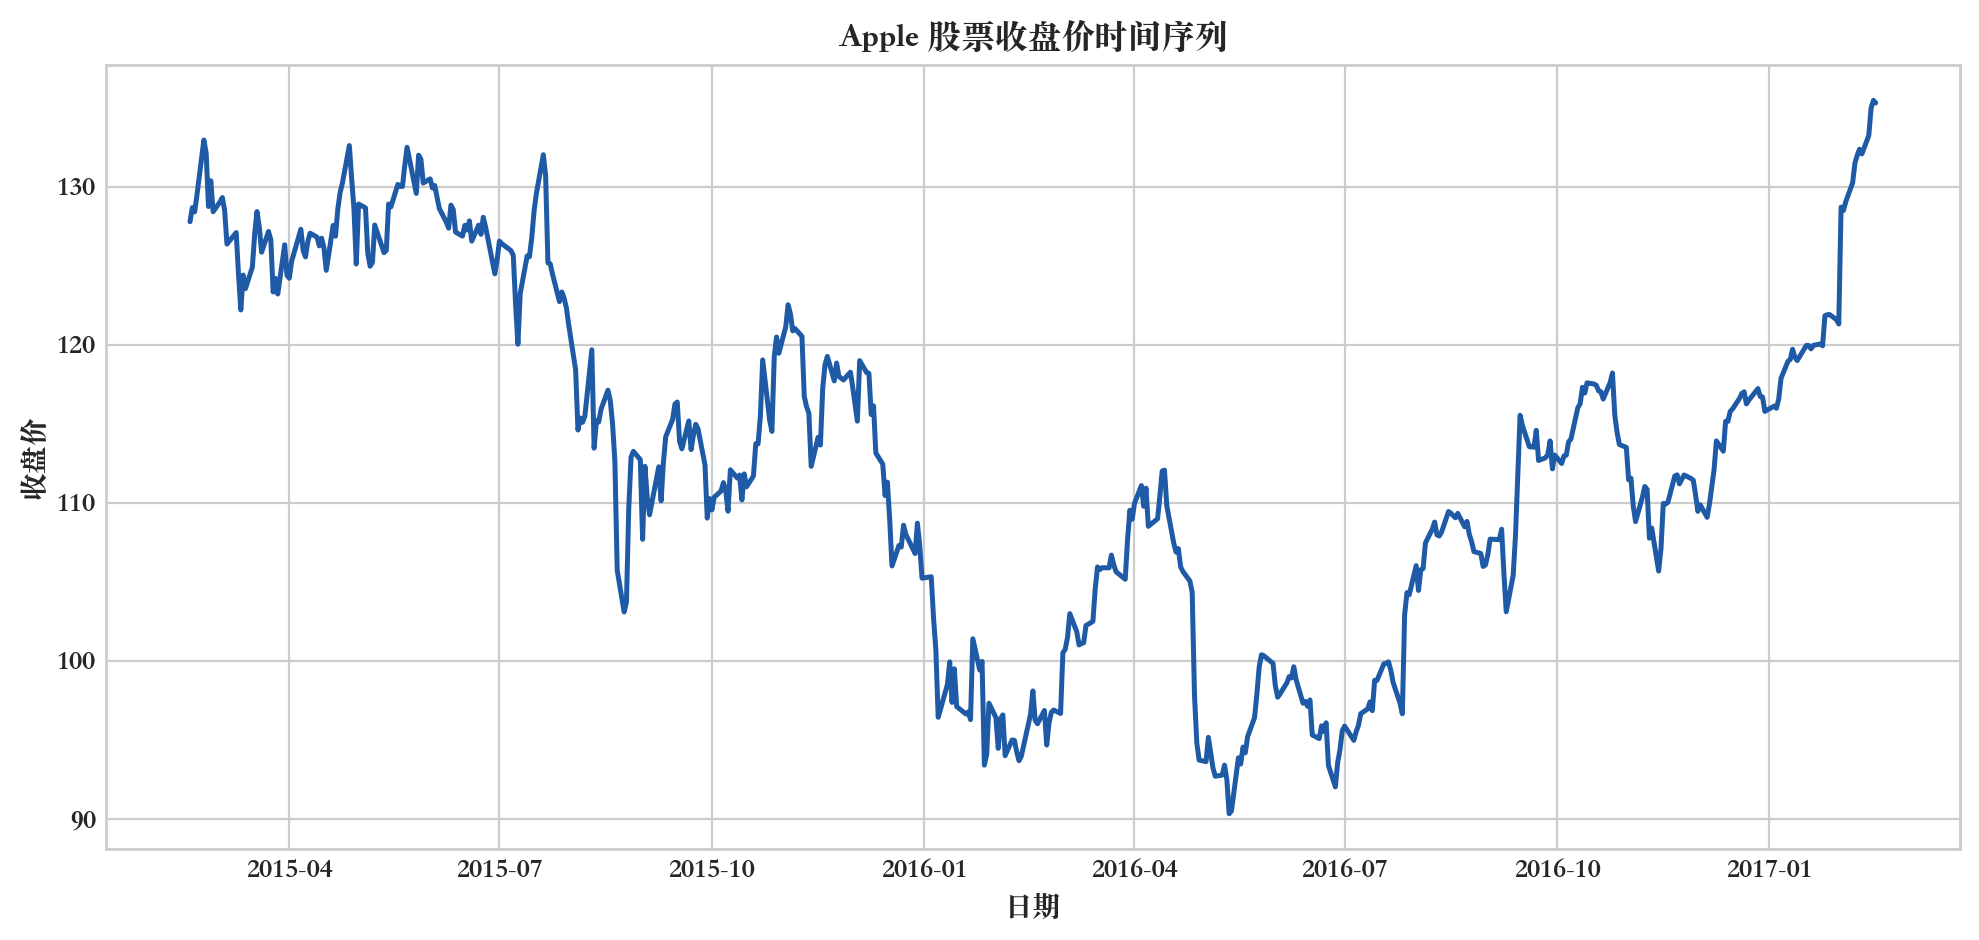
\includegraphics[width=0.88\textwidth]{outputs/figures/raw_close_series.png}
\caption{原始收盘价时间序列}
\end{figure}

\begin{figure}[H]
\centering
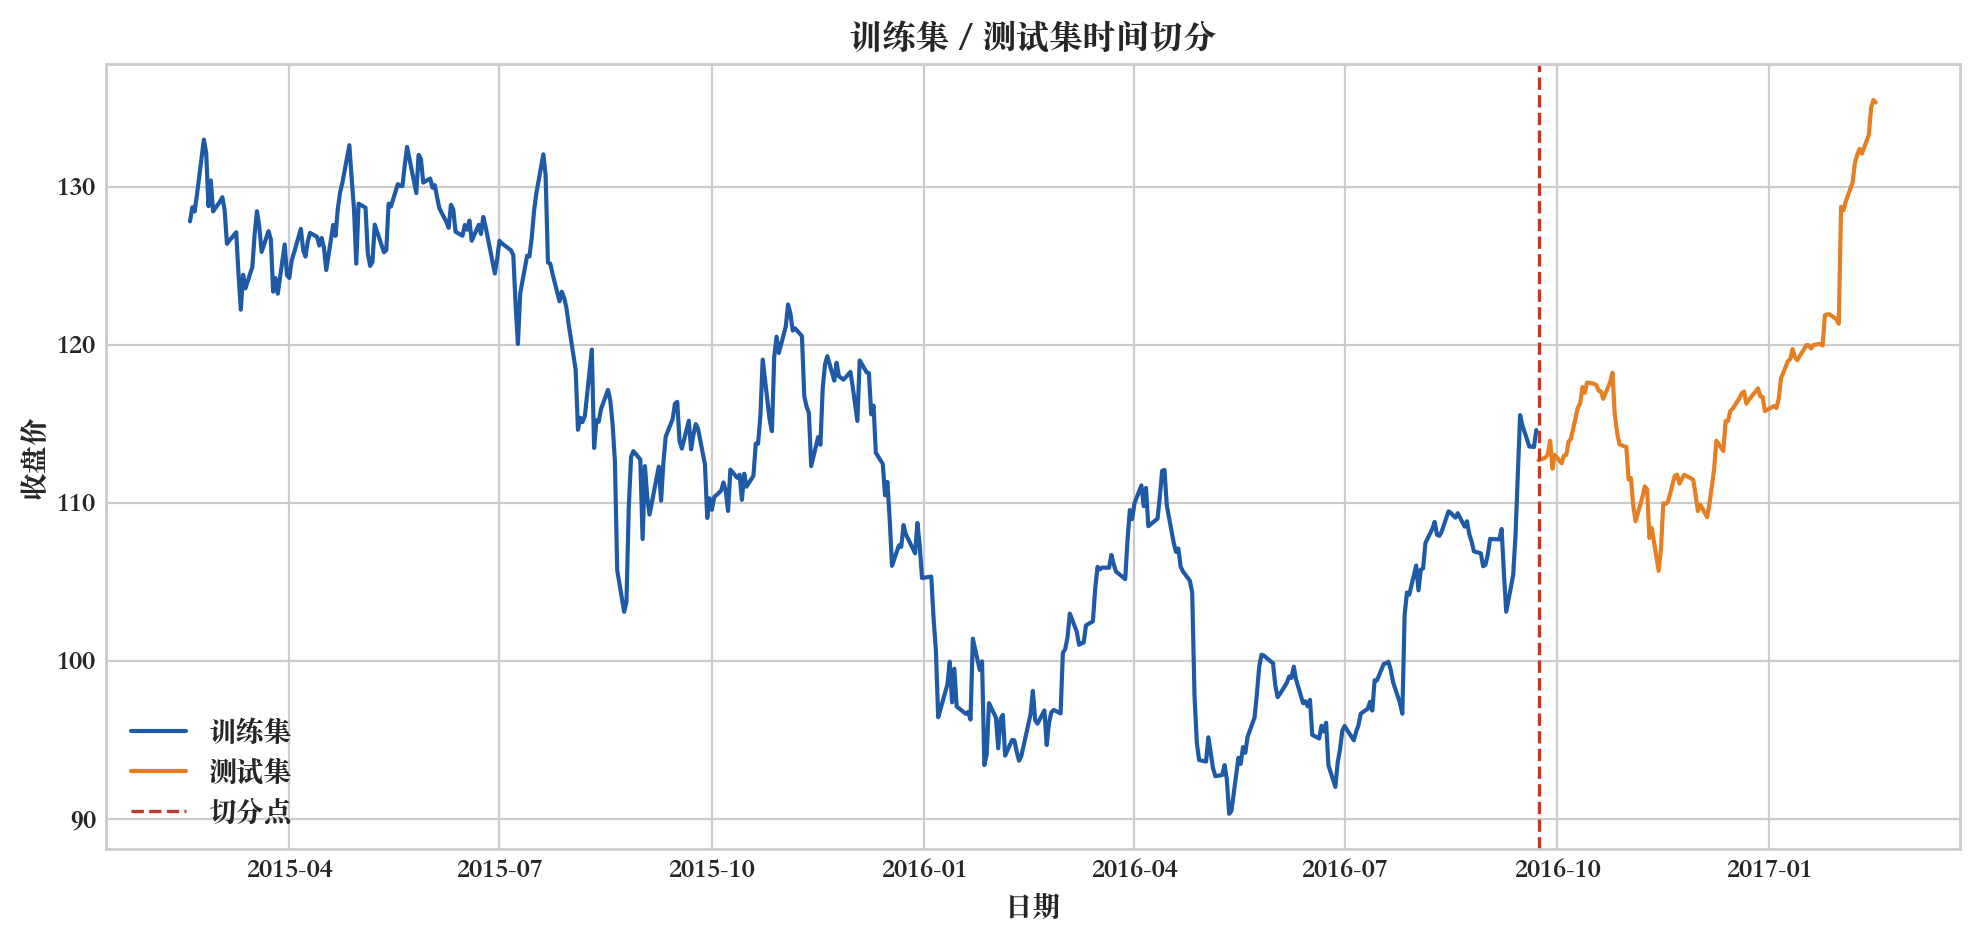
\includegraphics[width=0.88\textwidth]{outputs/figures/train_test_split.png}
\caption{训练集与测试集切分}
\end{figure}

\begin{figure}[H]
\centering
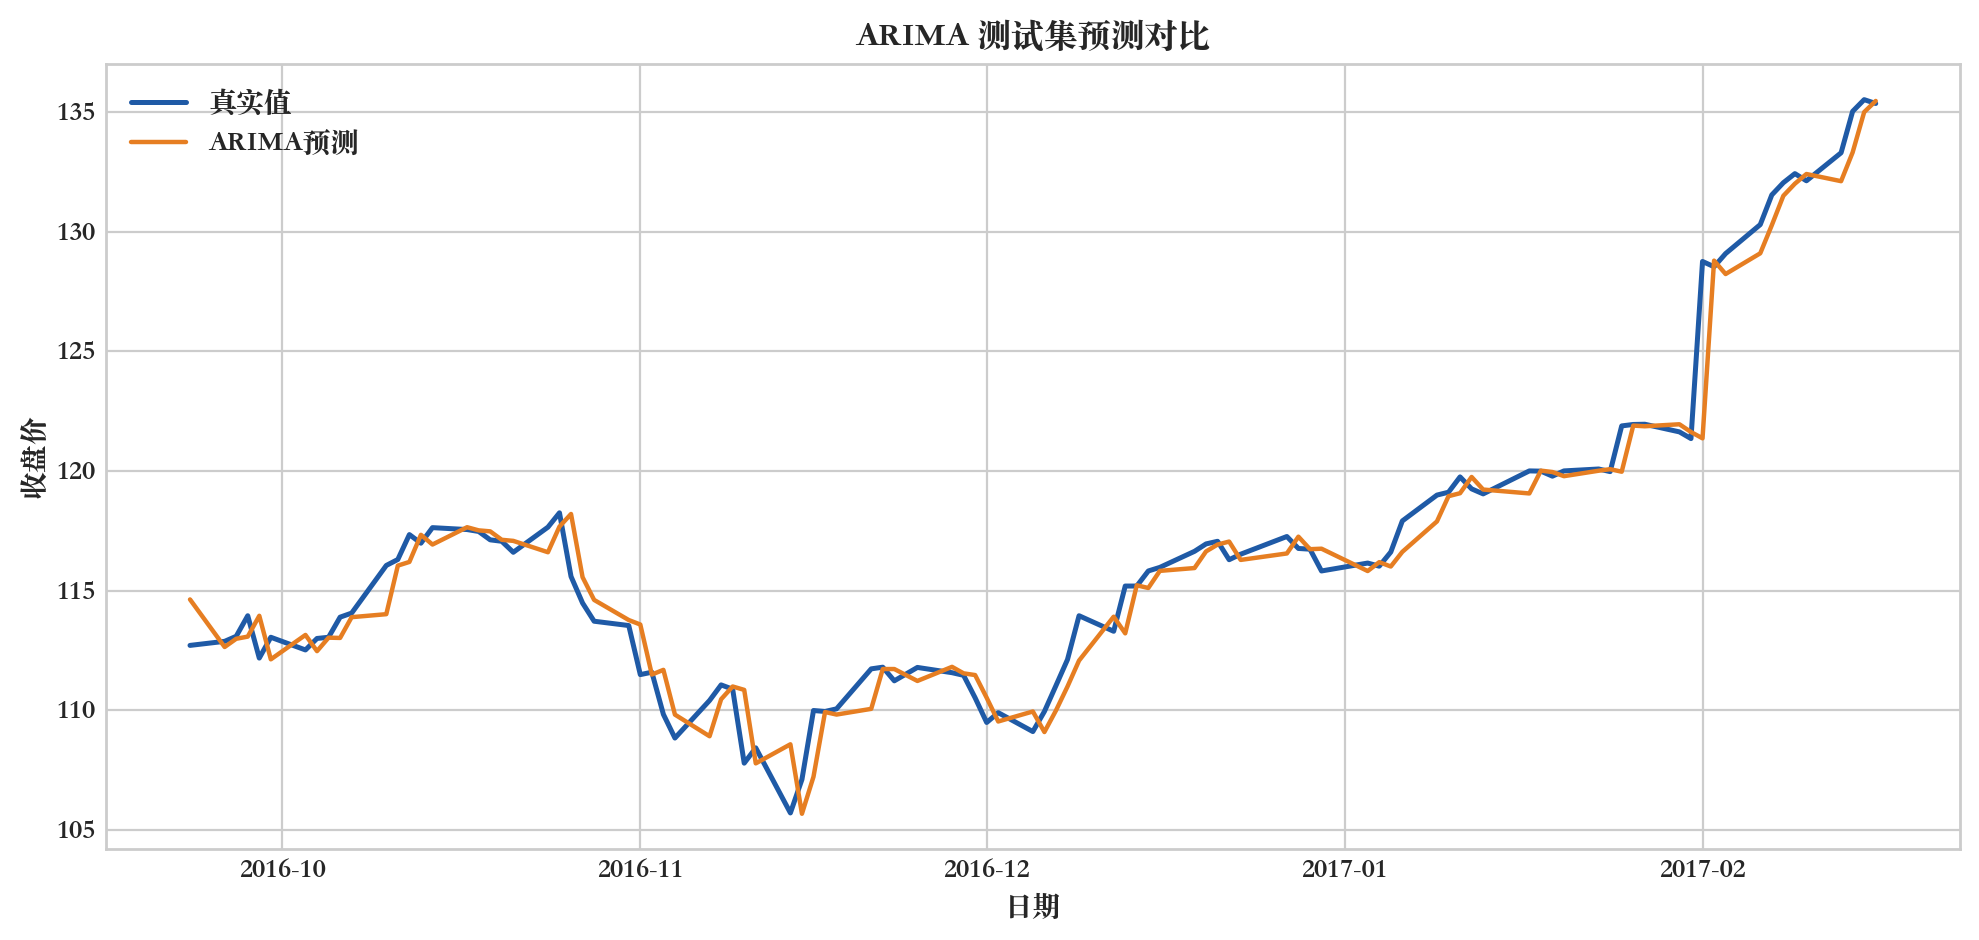
\includegraphics[width=0.88\textwidth]{outputs/figures/arima_vs_actual.png}
\caption{ARIMA 测试集预测对比}
\end{figure}

\begin{figure}[H]
\centering
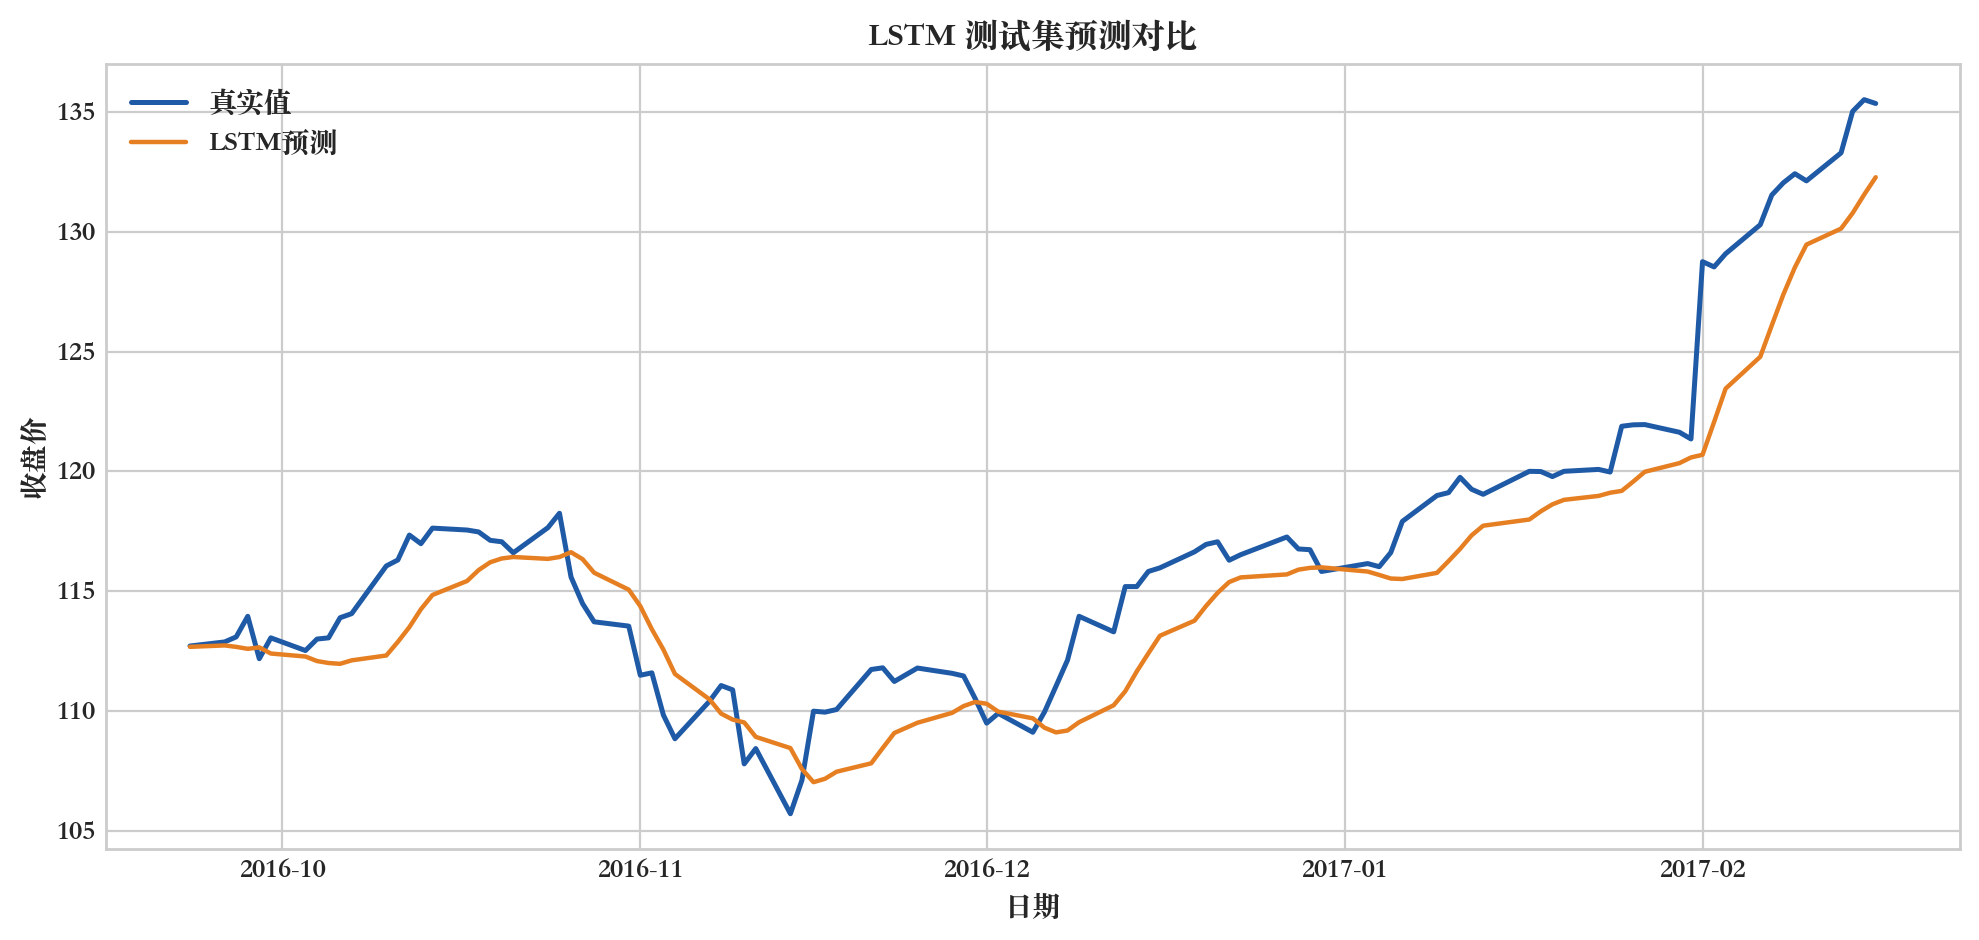
\includegraphics[width=0.88\textwidth]{outputs/figures/lstm_vs_actual.png}
\caption{LSTM 测试集预测对比}
\end{figure}

\begin{figure}[H]
\centering
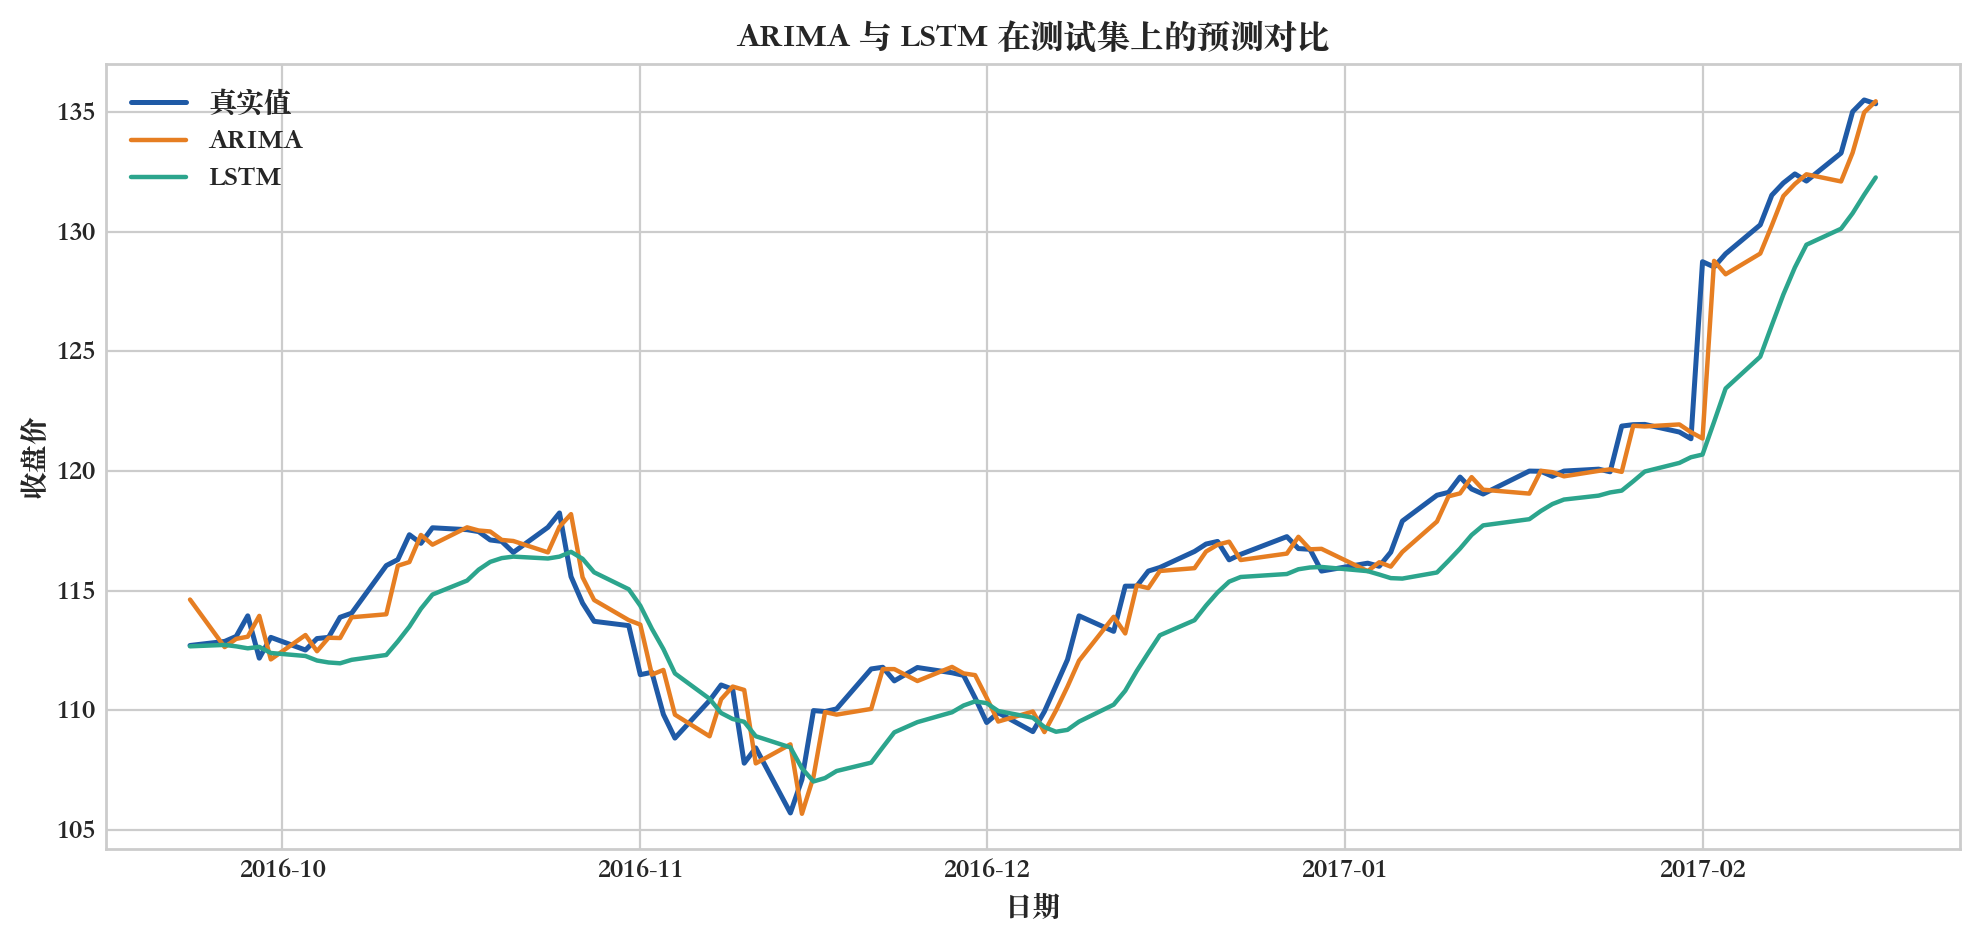
\includegraphics[width=0.88\textwidth]{outputs/figures/model_comparison.png}
\caption{两模型测试集预测综合对比}
\end{figure}

\begin{figure}[H]
\centering
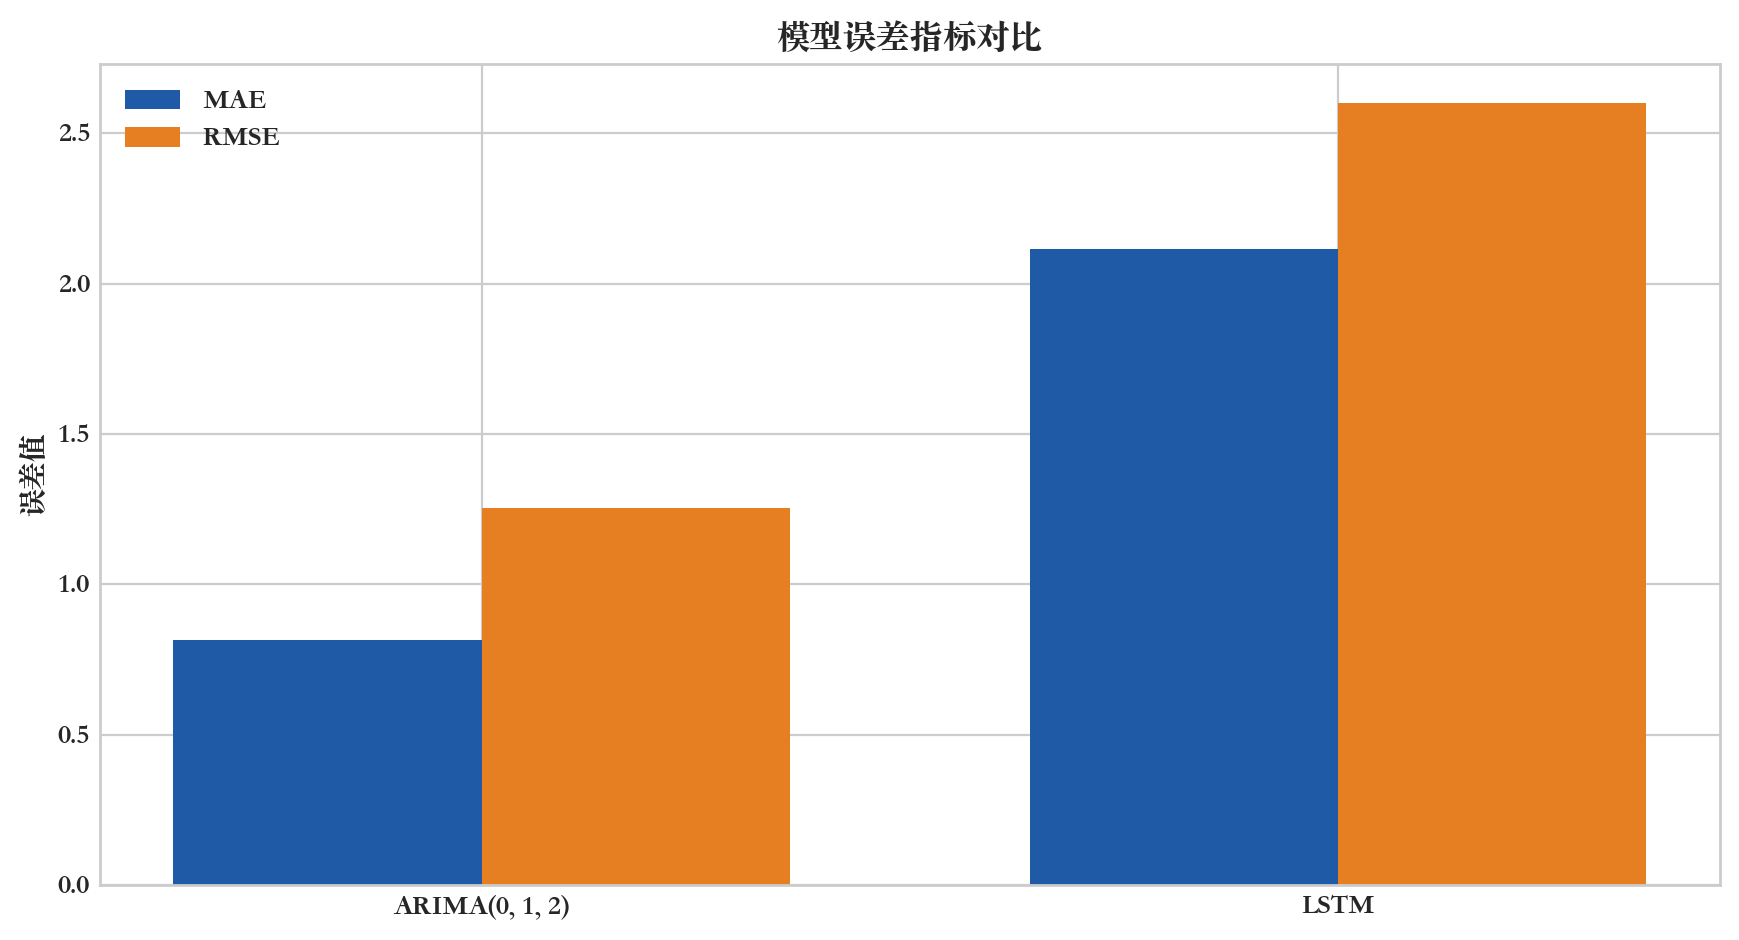
\includegraphics[width=0.78\textwidth]{outputs/figures/error_bar_chart.png}
\caption{MAE 与 RMSE 指标对比}
\end{figure}

\begin{figure}[H]
\centering
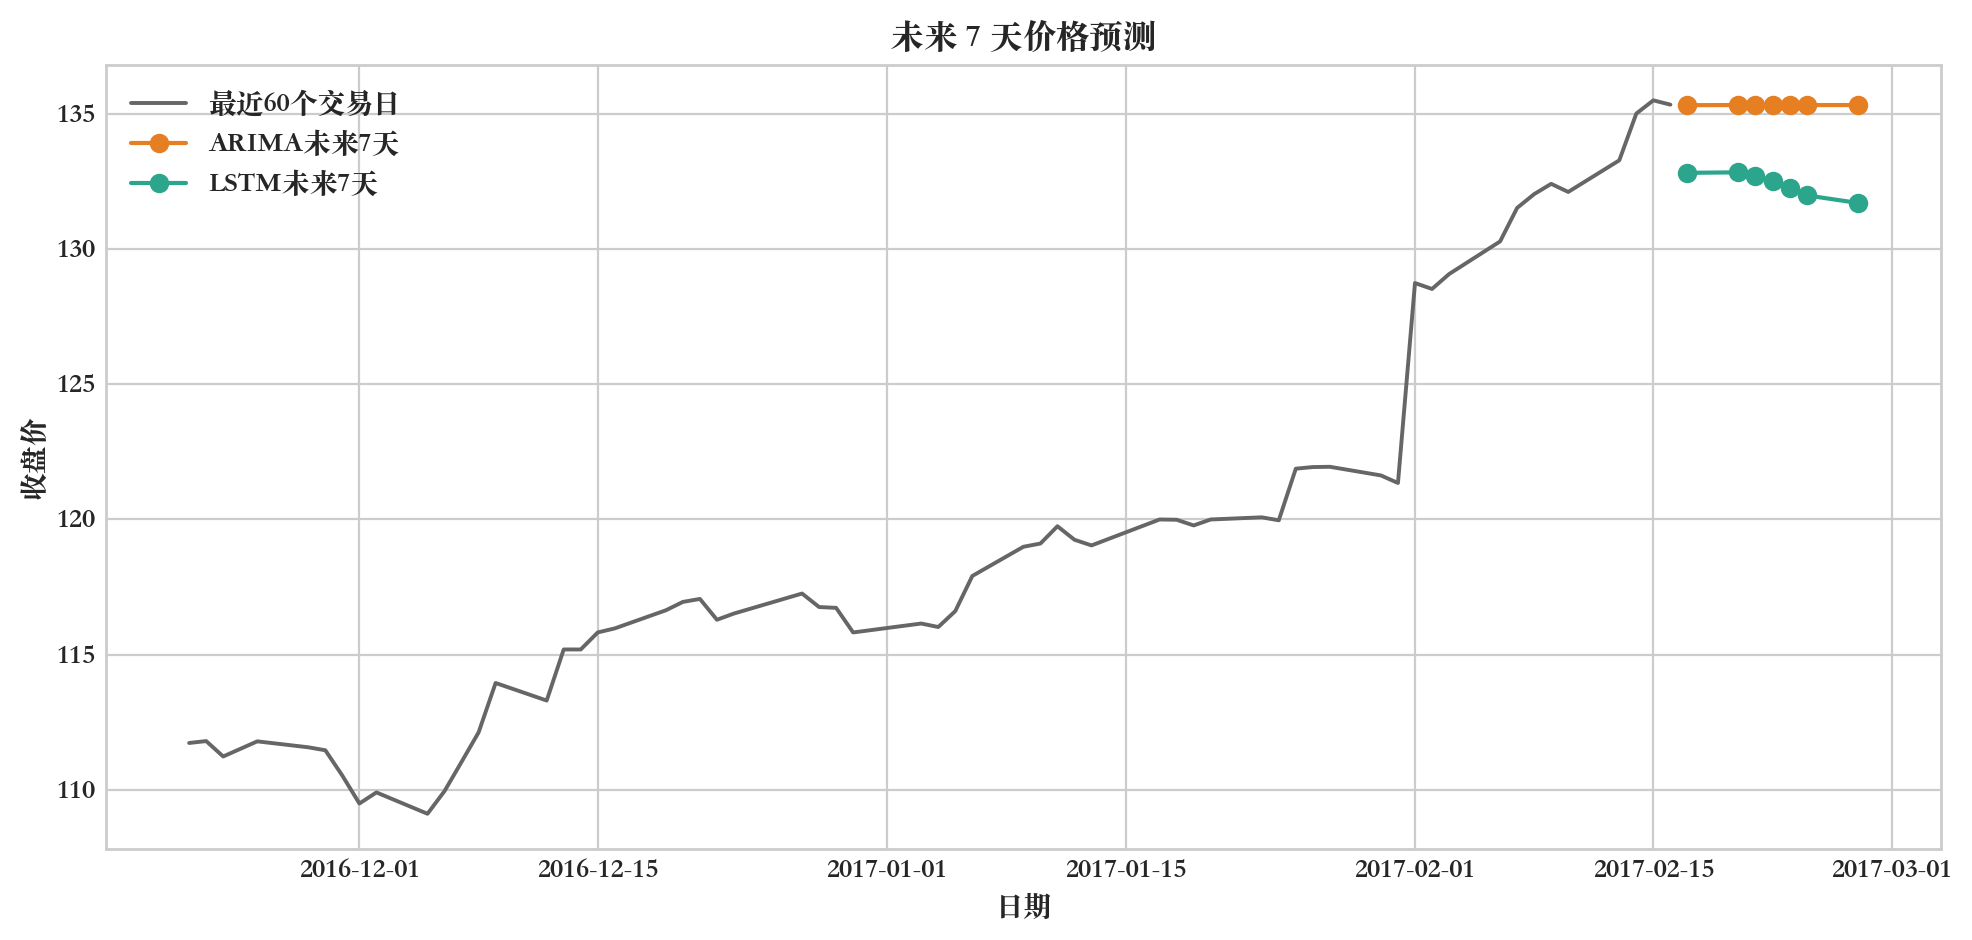
\includegraphics[width=0.88\textwidth]{outputs/figures/future_7days_forecast.png}
\caption{未来 7 天价格预测}
\end{figure}

\section{结果分析}
从误差指标可以直接看出，当前实验中 ARIMA 的表现明显优于 LSTM。具体而言，ARIMA(0,1,2) 在测试集上的 MAE 为 0.8137、RMSE 为 1.2547，而 LSTM 的 MAE 为 2.1156、RMSE 为 2.5984。两项指标均显示 ARIMA 的预测误差约为 LSTM 的一半左右，说明在本数据集和当前实验设置下，ARIMA 对收盘价短期波动的刻画更加准确。

结合测试集对比图也可以发现，采用滚动预测后，ARIMA 能够更紧密地跟随真实价格走势，尤其在局部上升、回落和平台阶段都保持了较好的同步性。相比之下，LSTM 的预测曲线虽然总体趋势正确，但存在更明显的滞后和平滑现象，对短期突变的响应不如 ARIMA 灵敏。

这种结果具有明确的工程合理性。当前任务是单变量、短期、低维的时间序列预测，样本规模也较小，这正是传统统计模型更容易发挥优势的场景。ARIMA 结构简单、参数可解释、训练速度快，在有限样本下仍能保持稳定性能。LSTM 作为深度学习模型，通常更依赖更大的数据规模、更长的训练时间以及更细致的超参数搜索；在本次仅使用 CPU、轻量网络和有限训练轮数的设置下，其优势尚未充分体现。

因此，就本次课程作业的目标而言，ARIMA 不仅是一个可运行的基线模型，而且是当前实验条件下更稳健、更准确、也更容易解释的方案；LSTM 则作为对照模型，展示了深度学习方法在时间序列建模中的另一条技术路线。

\section{实验结论}
本实验完成了课程作业要求的全部核心内容：股票历史 CSV 清洗、ARIMA 与 LSTM 两类模型实现、测试集误差对比、未来 7 天预测、图表输出以及 PDF 报告生成。综合实验结果可知，在当前数据规模与实验预算下，采用滚动预测的 ARIMA 在精度上明显优于 LSTM，并表现出更强的稳定性与可解释性，因此可以作为本次股票价格预测任务中更合适的主模型。LSTM 能够完整复现深度学习预测流程，但若要进一步超过 ARIMA，仍需要更多数据、更长训练时间以及更充分的参数调优。

\section{复现说明}
在 \texttt{作业5} 目录执行：
\begin{verbatim}
conda run -n ml python -m pip install -r requirements.txt
conda run -n ml python -m unittest discover -s tests -v
conda run -n ml python src/run_all.py
xelatex report.tex
xelatex report.tex
\end{verbatim}

\end{document}
